\documentclass{article}
\usepackage{graphicx}
\usepackage{amsmath}
\usepackage{parskip}
\title{Supporting Documentation for a Gyroscopic Fern}
\author{ijbd}
\begin{document}
	The goal of this iteration is to induce a new sense of wonder and curiosity in observers, 
	not just in the art that is produced (if my art can ever have that effect), but in the fundamental mechanics that drive Fern.
	With enough development, my hope is that people will scratch their heads to understand exactly how this machine moves.

	To accomplish our goal, we will replace the stacked linear axes with a pair of rotating arms (\ref{fig:high-level-concept}).
	We will put a motor on the end of each arm with a weighted ring to provide inertia.
	By changing the speed of the motor, we will change the angular momentum of the spinning rings,
	and, to conserve angular momentum, the arms will begin to rotate. 

	\begin{figure}[h!]
   		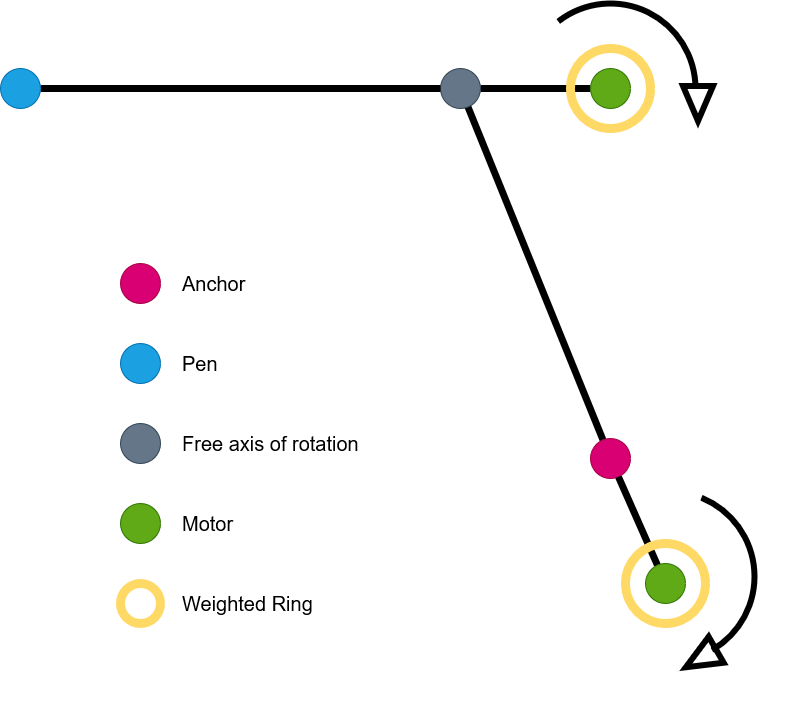
\includegraphics[width=\linewidth]{../diagrams/fern-v3-concept-diagram.png}   
		\caption{Birds-eye concept drawing of a gyroscopic fern.}
		\label{fig:high-level-concept}
	\end{figure}

	This document serves as theoretical foundation and proof-of-concept for this idea.
	To begin, we'll consider the case of a single arm.
	We'll assume the motor and supporting arms are massless.
	Let us start with the system at rest. The angular momentum is zero. 
	Suppose we begin spinning the motor such that the angular rotation about the rotor axis is $\omega$.
	We want to know what the resulting motion of the arm will be. 
	The conservation of angular momentum says that the change in angular momentum of a system (lacking any external torques)
	is zero. Therefore, we can express the rotational velocity of the arm as a function of the [change in] speed of the motor by equating
	the [change in] angular momentum of the motor with the angular momentum of the arm.

	First, we'll express the angular momentum of the spinning ring.

	By definition...
	\begin{align}
		L &= \vec{r} \times\vec{p}
	\end{align}

	Therefore..
	\begin{align}
		L &= \vec{r} \times m \vec{v} \\
		 &= \int_m\vec{r}\times\vec{v} dm \\
		 &= \int_{\theta}\vec{r}\times\rho\vec{v} d\theta
	\end{align}

	Where...
	\begin{align}
		\rho &= \frac{m_1}{2\pi}
	\end{align}
	And...
	\begin{align}
		L &= \rho\int_0^{2\pi}|\vec{r}(\theta)||\vec{v}|sin(\phi(\theta))d\theta
	\end{align}

	Where..
	\begin{align}
		\phi &= \angle\vec{v} - \angle\vec{r}
	\end{align}

	Solving for the needed quanitities...
	\begin{align}
		|\vec{r}(\theta)| &= \sqrt{R_1^2 + d_1^2 -2R_1d_1cos(\theta)} \\
		|\vec{v}| &= \omega r\\
		\phi(\theta) &= \frac{\pi}{2}-\theta-\alpha(\theta)
	\end{align}

	Where...
	\begin{align}
		\alpha &= \angle\vec{r}\\
		 &= sin^{-1}(\frac{R_1sin(\theta)}{|\vec{r}(\theta)|})
	\end{align}

	Continuing...
	\begin{align}
		sin(\phi(\theta)) &= sin(\frac{\pi}{2}-(\theta+\alpha(\theta)))
	\end{align}

	To simplify...
	\begin{align}
		sin(\phi(\theta)) &= cos(\theta + \alpha(\theta)) \\
		 &= cos(\theta)cos(\alpha(\theta)) - sin(\theta)sin(\alpha(\theta)) \\
		 &= cos(\theta)cos(sin^{-1}(\frac{R_1sin(\theta)}{|\vec{r}(\theta)|})) - sin(\theta)sin(sin^{-1}(\frac{R_1sin(\theta)}{|\vec{r}(\theta)|})) \\
		 &= cos(\theta)\sqrt{1-\frac{R_1^2sin^2(\theta)}{|\vec{r}(\theta)|^2}} - \frac{R_1}{|\vec{r}(\theta)|}sin^2(\theta) \\
		 &= cos(\theta)\sqrt{\frac{|\vec{r}(\theta)|^2 - R_1^2sin^2(\theta)}{|\vec{r}(\theta)|^2}} - \frac{R_1}{|\vec{r}(\theta)|}sin^2(\theta) \\
		 &= cos(\theta)\sqrt{\frac{R_1^2+d_1^2-2R_1d_1cos(\theta)- R_1^2sin^2(\theta)}{|\vec{r}(\theta)|^2}} - \frac{R_1}{|\vec{r}(\theta)|}sin^2(\theta) \\
		 &= cos(\theta)\sqrt{\frac{R_1^2(1-sin^2(\theta))+d_1^2-2R_1d_1cos(\theta)}{|\vec{r}(\theta)|^2}} - \frac{R_1}{|\vec{r}(\theta)|}sin^2(\theta) \\
		 &= cos(\theta)\sqrt{\frac{R_1^2cos^2(\theta)+d_1^2-2R_1d_1cos(\theta)}{|\vec{r}(\theta)|^2}} - \frac{R_1}{|\vec{r}(\theta)|}sin^2(\theta) \\
		 &= cos(\theta)\sqrt{\frac{(R_1cos(\theta) - d_1)^2}{|\vec{r}(\theta)|^2}} - \frac{R_1}{|\vec{r}(\theta)|}sin^2(\theta) \\
		 &= \frac{d_1cos(\theta) - R_1cos^2(\theta) - R_1sin^2(\theta)}{|\vec{r}(\theta)|} \\
		 &= \frac{d_1cos(\theta) - R_1(cos^2(\theta) + sin^2(\theta))}{|\vec{r}(\theta)|} \\
		 &= \frac{d_1cos(\theta) - R_1}{|\vec{r}(\theta)|}
	\end{align}
	Recall...
	\begin{align}
		L &= \rho\int_0^{2\pi}|\vec{r}(\theta)||\vec{v}|sin(\phi(\theta))d\theta
	\end{align}

	Finally...
	\begin{align}
		L &=\rho\omega R_1\int_0^{2\pi}|\vec{r}(\theta)|\frac{d_1cos(\theta) - R_1}{|\vec{r}(\theta)|}d\theta \\
		 &= \rho\omega R_1\int_0^{2\pi}d_1cos(\theta) - R_1 d\theta \\
		 &= \rho\omega R_1^2 2\pi \\
		 &= \frac{m}{2\pi} \omega R_1^2 2\pi  \\
		 &= m \omega R_1^2
	\end{align}

	dd
	
\end{document}
